% =====================================================================
%  Uniworld — preamble
%  Identity, type system and page furniture.
%  Every field here is fixed by the owner except \bookDOI, which is
%  per-book and lives in exactly one place so it can be swapped in
%  a single edit.
%
%  There is no published source repository for this book. A code link
%  belongs in the book only if the owner supplies one for that title.
%  Typeset with XeLaTeX.
% =====================================================================

% ---- Standing book identity -------------------------------------------
\newcommand{\bookTitle}{Is the Riemann Hypothesis Solved?}
\newcommand{\bookSubtitle}{A Critical Audit of the Lean Formalization, the Theta-Lift Method, and the Two-Thirds Ceiling}
\newcommand{\bookAuthor}{Gerald Enrique Nelson Mc Kenzie}
\newcommand{\bookImprint}{Tico Internet LLC}
\newcommand{\bookEdition}{2026 First Edition}
\newcommand{\bookLicense}{Apache License 2.0}
\newcommand{\bookDOI}{10.5281/zenodo.24408811}   % <-- the one field that changes
\newcommand{\bookFactsDate}{21 November 2026}
\newcommand{\bookCopyright}{2026}

% =====================================================================
%  Colour engine — loaded first, the tokens below need it
\usepackage[table]{xcolor}

% =====================================================================
%  DESIGN TOKENS
%  One palette, one type system. Change a value here and the whole
%  book follows.
% =====================================================================
% Palette — a dark instrument panel: ink ground, phosphor accent,
% amber reserved for warnings and caveats.
\definecolor{dbg}{HTML}{0C1016}        % page background
\definecolor{panel}{HTML}{151D27}      % card / table tint
\definecolor{paneledge}{HTML}{27333F}  % card border, hairlines
\definecolor{accent}{HTML}{8FD6C0}     % the single accent
\definecolor{accentdim}{HTML}{4C7D70}  % accent at low emphasis
\definecolor{txt}{HTML}{E6EBEF}        % body text
\definecolor{txtdim}{HTML}{8B9BA7}     % secondary text, captions, folios
\definecolor{gridline}{HTML}{1A222C}   % background grid
\definecolor{amber}{HTML}{E0A458}      % used only for the one accent note

% Type scale (points) — sizes follow the design system, not habit
\newcommand{\szDisplay}{30}    % cover title
\newcommand{\szTitle}{17}        % part / chapter title
\newcommand{\szSection}{12.4}      % section
\newcommand{\szSub}{10.6}      % subsection
\newcommand{\szBody}{10.2}     % body
\newcommand{\szCaption}{8.2}   % captions
\newcommand{\szMeta}{7.4}     % running heads, folios

% ---- Package stack ------------------------------------------------------
\usepackage{fontspec}
\usepackage{unicode-math}
\setmainfont{Outfit}[
  UprightFont={Outfit Regular}, BoldFont={Outfit Bold},
  ItalicFont={Outfit Regular}, ItalicFeatures={FakeSlant=0.20},
  BoldItalicFont={Outfit Bold}, BoldItalicFeatures={FakeSlant=0.20},
  Ligatures={TeX}]
\setsansfont{Outfit}[
  UprightFont={Outfit Regular}, BoldFont={Outfit Bold},
  ItalicFont={Outfit Regular}, ItalicFeatures={FakeSlant=0.20},
  BoldItalicFont={Outfit Bold}, BoldItalicFeatures={FakeSlant=0.20},
  Ligatures={TeX}]
% The book's code face is DejaVu Sans Mono rather than JetBrains Mono: the
% quotations from the submitted Lean source contain characters (U+207B, U+1D41,
% U+2229, U+211D) that JetBrains Mono does not carry, and the alternative
% would be to alter a quoted source. DejaVu covers the full set.
\setmonofont{DejaVu Sans Mono}[
  UprightFont={DejaVu Sans Mono}, BoldFont={DejaVu Sans Mono Bold},
  ItalicFont={DejaVu Sans Mono}, BoldItalicFont={DejaVu Sans Mono Bold},
  ItalicFeatures={FakeSlant=0.20}, BoldItalicFeatures={FakeSlant=0.20},
  Ligatures={TeX}]
% Fira Math ships a single weight in this TeX Live installation. The book
% uses no bold mathematics, so bold maps to the regular face; if bold maths
% is ever added, install FiraMath-Bold and point BoldFont at it.
\setmathfont{FiraMath-Regular.otf}[
  Path=/usr/share/texlive/texmf-dist/fonts/opentype/public/firamath/,
  Extension = .otf, Ligatures = {TeX}, Scale = 1.0,
  BoldFont = FiraMath-Regular.otf]

\usepackage{textcomp}
\usepackage{amsmath,bm}
\usepackage{ragged2e}
\usepackage{fvextra}
% The Lean quotations contain characters the book's code face does not carry
% (U+207B, U+1D41, U+2229, U+211D). The listings are therefore set in a
% monospace with the full coverage, so that a quoted source is never
% silently altered to make it fit. The switch is local to the listing, so
% the inline code face is unchanged.
% Lean code is quoted verbatim from the submission and many lines are far
% wider than a 6 x 9 text column. fvextra's line breaking is what keeps those
% quotes inside the measure instead of running off the page.
\fvset{
  breaklines=true,
  breakanywhere=true,
  breaksymbolleft={},
  breaksymbolright={},
  fontsize=\footnotesize,
  baselinestretch=1.0
}
% A quotation from the submitted source. fancyvrb resets the face to the
% default monospace on entry, so the family is swapped locally instead.
\DefineVerbatimEnvironment{leanquote}{Verbatim}{
  fontsize=\footnotesize,
  breaklines=true,
  breakanywhere=true,
  breaksymbolleft={},
  fontfamily=tt
}
\RecustomVerbatimEnvironment{verbatim}{Verbatim}{
  breaklines=true,
  breakanywhere=true,
  breaksymbolleft={},
  breaksymbolright={},
  fontsize=\footnotesize
}
% XeTeX performs character protrusion itself, from the font's own tables.
% microtype's protrusion tables are meant for pdfTeX, and its inheritance
% list for the TU encoding asks for slots that a Unicode encoding does not
% provide, so it warns twice about characters it never sets here. Turning
% microtype's own protrusion off leaves the engine's protrusion in place and
% the warning out of the log; the typesetting is byte for byte the same.
\usepackage[protrusion=false]{microtype}
\usepackage{graphicx}
\usepackage{tikz}
\usepackage{pgfplots}
\usepackage{booktabs}
\usepackage{tabularx}
\usepackage{longtable}
\usepackage{array}
\usepackage{multirow}
\usepackage{makecell}
\usepackage{enumitem}
\usepackage{float}
\usepackage{caption}
\usepackage{tcolorbox}
\tcbuselibrary{skins,breakable}
\usepackage{fancyhdr}
\usepackage{titlesec}
\usepackage{tocloft}
\usepackage{pdfpages}
\usepackage{eso-pic}
% Long file paths are quoted from the submission and are far wider than a
% 6 x 9 measure; \path breaks them at slashes instead of running off.
\usepackage{url}
\urlstyle{tt}
\usepackage{seqsplit}
% Long Lean identifiers have no break opportunity of their own.
% \code breaks them between characters.
\newcommand{\code}[1]{\texttt{\seqsplit{#1}}}
\usepackage{hyperref}
\usepackage{makeidx}
\usepackage[english]{babel}

\pgfplotsset{compat=1.18}

% ---- Page geometry: 6 x 9 in trim --------------------------------------
\usepackage[
  paperwidth=6in, paperheight=9in,
  inner=0.80in, outer=0.60in,
  top=0.82in, bottom=0.78in,
  headheight=14pt, headsep=16pt,
  footskip=28pt
]{geometry}

% ---- Page colour -------------------------------------------------------
\pagecolor{dbg}
\color{txt}

% ---- Paragraph and list rhythm -----------------------------------------
\setlength{\parindent}{0pt}
\setlength{\parskip}{5.5pt plus 1pt}
\linespread{1.06}
\raggedbottom
\widowpenalty=10000
\clubpenalty=10000
\sloppy

\setlist[itemize]{leftmargin=1.15em,itemsep=3.5pt,topsep=4pt,parsep=0pt,
  label=\textcolor{accent}{\textbullet}}
\setlist[enumerate]{leftmargin=1.45em,itemsep=3.5pt,topsep=4pt,parsep=0pt,
  label=\textcolor{accent}{\ttfamily\theenumi.}}
\renewcommand{\labelitemii}{\textcolor{accent}{\textendash}}

% ---- Background grid for openers ---------------------------------------
% The grid motif appears on part and chapter openers only: it reads as
% design there, and as noise behind body text. Coordinates are in inches,
% measured from the lower-left corner of the page.
\newcommand{\gridlayer}{%
  \AddToShipoutPictureBG*{%
    \AtPageLowerLeft{%
      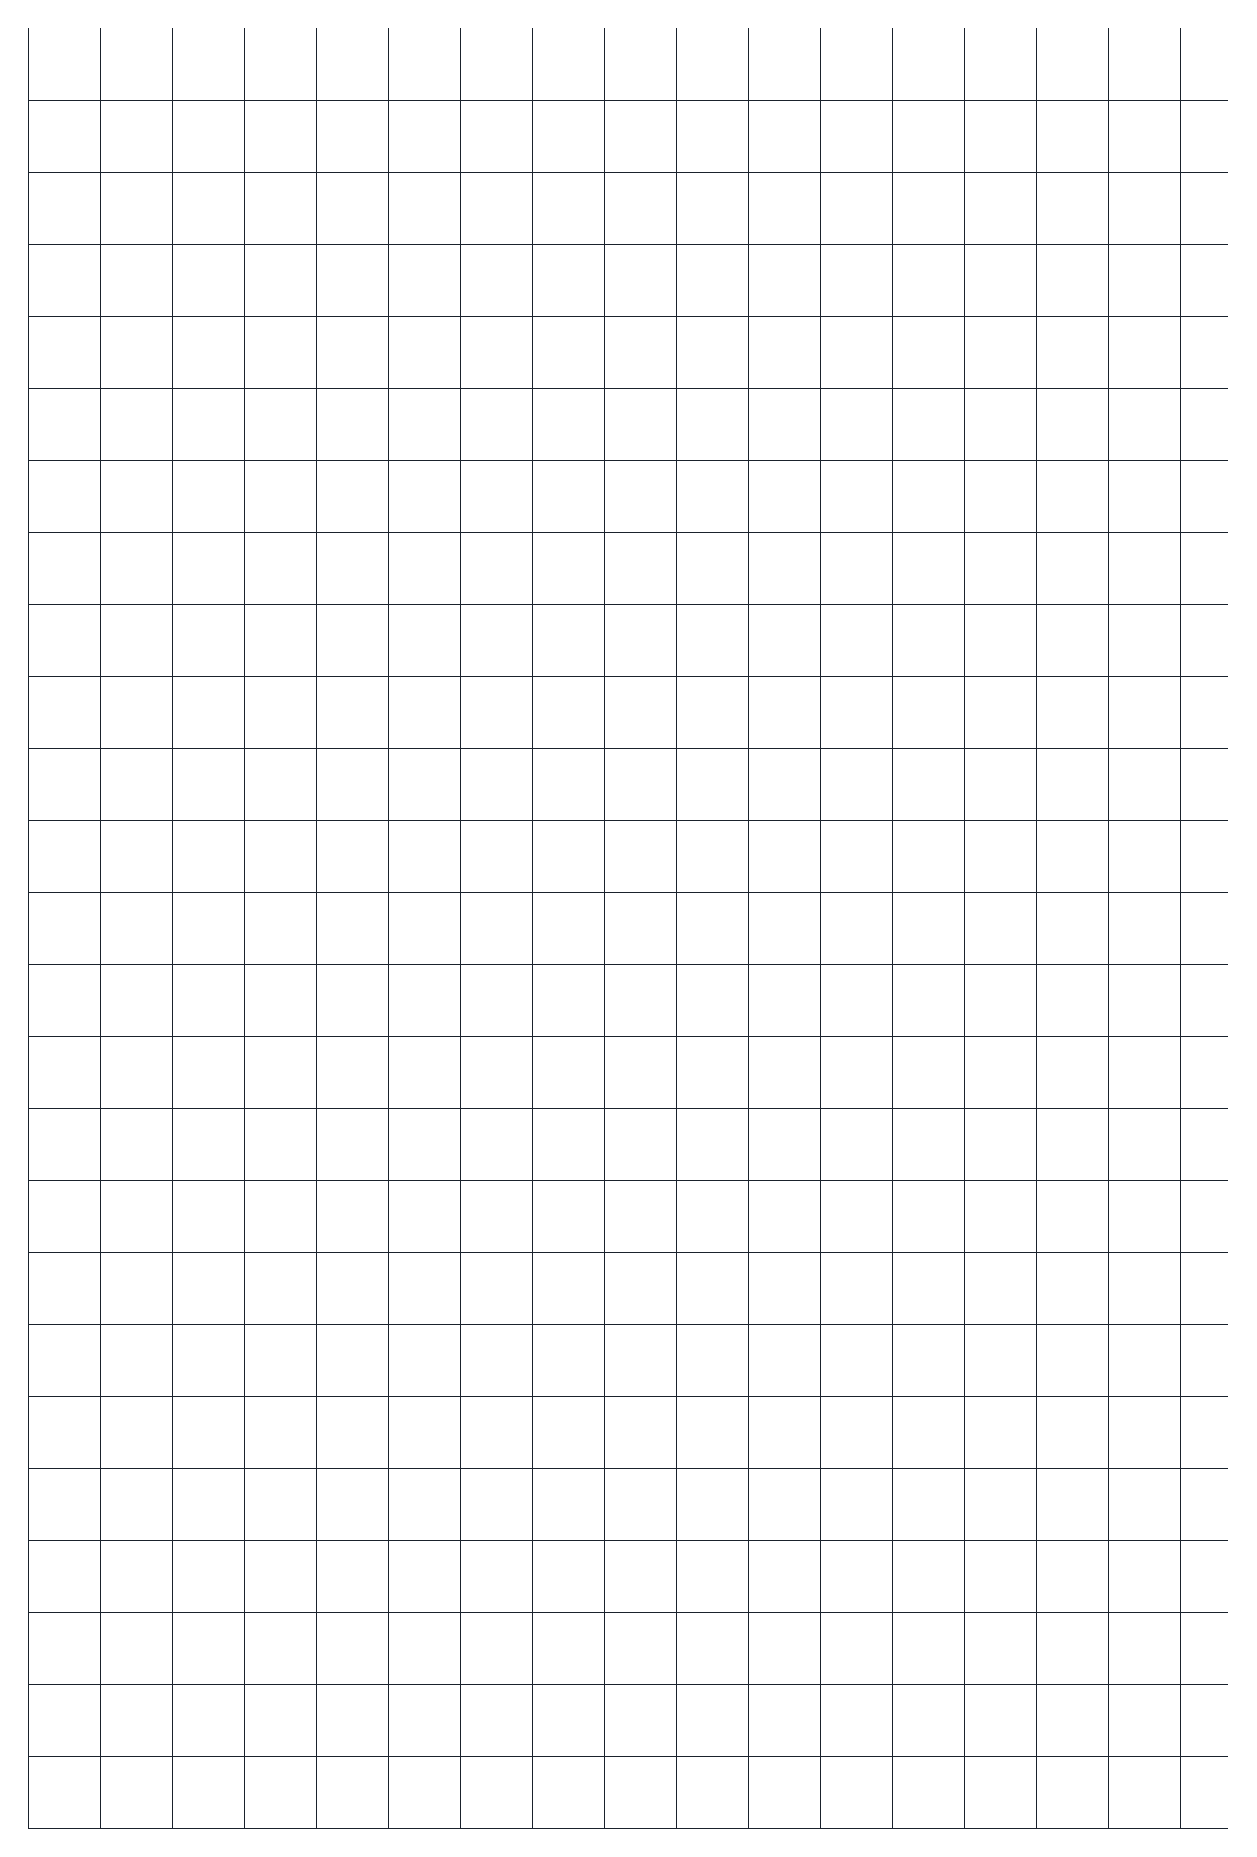
\begin{tikzpicture}[x=1in,y=1in]
        \foreach \yy in {0,0.36,...,9.0}{%
          \draw[color=gridline,line width=0.3pt] (0,\yy) -- (6,\yy);}
        \foreach \xx in {0,0.36,...,6.0}{%
          \draw[color=gridline,line width=0.3pt] (\xx,0) -- (\xx,9);}
      \end{tikzpicture}}}}

% ---- Headings -----------------------------------------------------------
\titleformat{\part}[display]
  {\normalfont\sffamily\bfseries\raggedright\color{txt}\vspace*{1.15in}\gridlayer\thispagestyle{opener}}
  {\ttfamily\fontsize{9.5}{11}\selectfont\color{accent}\MakeUppercase{Part \thepart}}
  {9pt}{\fontsize{\szTitle}{20}\selectfont\color{txt}}
  [\vspace{14pt}\textcolor{accent}{\rule{\textwidth}{1.6pt}}]
\titlespacing*{\part}{0pt}{0pt}{30pt}

\titleformat{\chapter}[display]
  {\normalfont\sffamily\bfseries\raggedright\color{txt}\gridlayer\thispagestyle{opener}}
  {\ttfamily\fontsize{9.5}{11}\selectfont\color{accent}\MakeUppercase{Chapter \thechapter}}
  {7pt}{\fontsize{\szTitle}{20}\selectfont\color{txt}}
  [\vspace{10pt}\textcolor{accent}{\rule{\textwidth}{1.6pt}}]
\titlespacing*{\chapter}{0pt}{-0.10in}{22pt}

\titleformat{\section}
  {\sffamily\bfseries\color{txt}}
  {\textcolor{accent}{\ttfamily\large\thesection}}{0.6em}{}
\titlespacing*{\section}{0pt}{16pt}{7pt}

\titleformat{\subsection}
  {\sffamily\bfseries\color{txt}}
  {\textcolor{accent}{\ttfamily\normalsize\thesubsection}}{0.55em}{}
\titlespacing*{\subsection}{0pt}{12pt}{5pt}

\titleformat{\subsubsection}
  {\sffamily\bfseries\color{txtdim}}
  {\textcolor{accentdim}{\ttfamily\small\thesubsection}}{0.5em}{}
\titlespacing*{\subsubsection}{0pt}{10pt}{4pt}

% ---- Contents, figures, tables -----------------------------------------
\renewcommand{\cftpartfont}{\ttfamily\bfseries\large\color{accent}}
\renewcommand{\cftchapfont}{\sffamily\bfseries\normalsize\color{txt}}
\renewcommand{\cftsecfont}{\sffamily\normalsize\color{txtdim}}
\renewcommand{\cftpartpagefont}{\ttfamily\color{txtdim}}
\renewcommand{\cftchappagefont}{\ttfamily\color{txtdim}}
\renewcommand{\cftsecpagefont}{\ttfamily\color{txtdim}}
\setcounter{tocdepth}{1}
\renewcommand{\contentsname}{Contents}
\renewcommand{\partname}{Part}
\renewcommand{\listfigurename}{Figures}
\renewcommand{\listtablename}{Tables}
\renewcommand{\figurename}{Figure}
\renewcommand{\tablename}{Table}

% ---- Running heads and folios ------------------------------------------
\renewcommand{\chaptermark}[1]{\markboth{#1}{}}
\renewcommand{\partmark}[1]{\markboth{\MakeUppercase{Part \thepart}}{}}

\pagestyle{fancy}
\fancyhf{}
\renewcommand{\headrulewidth}{0pt}
\renewcommand{\footrulewidth}{0pt}
\fancyhead[LE]{\ttfamily\fontsize{\szMeta}{9}\selectfont\color{txtdim}%
  \MakeUppercase{\bookTitle}}
\fancyhead[RO]{\ttfamily\fontsize{\szMeta}{9}\selectfont\color{txtdim}%
  \MakeUppercase{\leftmark}}
\fancyfoot[C]{\ttfamily\fontsize{\szMeta}{9}\selectfont\color{txtdim}\thepage}
\renewcommand{\headrule}{\hbox to\headwidth{%
  \color{accentdim}\leaders\hrule height 0.35pt\hfill}}
\renewcommand{\footrulewidth}{0pt}

\fancypagestyle{plain}{%
  \fancyhf{}
  \renewcommand{\headrulewidth}{0pt}
  \fancyfoot[C]{\ttfamily\fontsize{\szMeta}{9}\selectfont\color{txtdim}\thepage}}

% Chapter and part openers: folio only, no running head.
\fancypagestyle{opener}{%
  \fancyhf{}
  \renewcommand{\headrulewidth}{0pt}
  \fancyfoot[C]{\ttfamily\fontsize{\szMeta}{9}\selectfont\color{txtdim}\thepage}}

% ---- Figure and table captions -----------------------------------------
\captionsetup{font=footnotesize,labelfont={tt,bf,color=accent},
  textfont={color=txtdim},labelsep=period,width=0.96\textwidth,
  justification=justified,singlelinecheck=false,skip=7pt}
% The per-type skips are set at the start of the document: issued in the
% preamble, before the caption package knows that a table and a figure
% caption type exist, they are reported as unused.
\AtBeginDocument{%
  \captionsetup[table]{skip=6pt}%
  \captionsetup[figure]{skip=7pt}}

% ---- Epigraph (the book class does not supply one) ----------------------
\providecommand{\epigraphname}{Epigraph}
\newenvironment{epigraph}{\begin{quotation}\small\itshape}{\end{quotation}}

% ---- Cards (callout boxes) ---------------------------------------------
% the roles
\newtcolorbox{takeaway}[1]{enhanced, breakable, colback=panel,
  colframe=paneledge, boxrule=0.5pt, leftrule=2.6pt, arc=0pt, outer arc=0pt,
  left=10pt, right=9pt, top=8pt, bottom=8pt,
  fonttitle=\ttfamily\bfseries\fontsize{8.2}{10}\selectfont, coltitle=accent,
  colbacktitle=panel, coltext=txt, title={#1}, before skip=12pt, after skip=12pt}
\newtcolorbox{mythbox}[1]{enhanced, breakable, colback=panel,
  colframe=paneledge, boxrule=0.5pt, leftrule=2.6pt, arc=0pt, outer arc=0pt,
  left=10pt, right=9pt, top=8pt, bottom=8pt,
  fonttitle=\ttfamily\bfseries\fontsize{8.2}{10}\selectfont, coltitle=txtdim,
  colbacktitle=panel, coltext=txt, title={#1}, before skip=12pt, after skip=12pt}
\newtcolorbox{deeper}[1]{enhanced, breakable, colback=panel,
  colframe=paneledge, boxrule=0.5pt, leftrule=1.1pt, arc=0pt, outer arc=0pt,
  left=10pt, right=9pt, top=8pt, bottom=8pt,
  fonttitle=\ttfamily\bfseries\fontsize{8.2}{10}\selectfont, coltitle=accentdim,
  colbacktitle=panel, coltext=txt, title={#1}, before skip=12pt, after skip=12pt}
\newtcolorbox{seamnote}[1]{enhanced, breakable, colback=panel,
  colframe=accent, boxrule=0.8pt, arc=0pt, outer arc=0pt,
  left=10pt, right=9pt, top=8pt, bottom=8pt,
  fonttitle=\ttfamily\bfseries\fontsize{8.2}{10}\selectfont, coltitle=accent,
  colbacktitle=panel, coltext=txt, title={#1}, before skip=12pt, after skip=12pt}

\newenvironment{keytakeaways}{%
  \begin{takeaway}{Key Takeaways}\small\begin{itemize}\setlength{\itemsep}{3pt}\setlength{\topsep}{3pt}\relax
}{%
  \end{itemize}\end{takeaway}%
}
\newenvironment{commonmyths}{%
  \begin{mythbox}{Common Myths, Straightened Out}\small\begin{itemize}\setlength{\itemsep}{3pt}\setlength{\topsep}{3pt}\relax
}{%
  \end{itemize}\end{mythbox}%
}

% ---- Math conveniences --------------------------------------------------
% FiraMath carries neither U+211C (REAL PART SYMBOL) nor U+229E (SQUARED
% PLUS). Left alone, both render as a missing-glyph box inside an equation.
% \Re is therefore set upright through \operatorname, and \boxplus is drawn,
% so that no equation in the book contains a replacement character.
% \Re and \boxplus are deliberately NOT used: the math font carries
% neither U+211C nor U+229E, and the font machinery reinstates them as
% literal characters, so they typeset as a missing-glyph box. \mathrm{Re}
% and \tboxplus are used instead and are set below.
\newcommand{\tboxplus}{\mathbin{%
  \tikz[baseline=-0.44ex,x=1ex,y=1ex,line width=0.5pt]{%
    \draw (0,0) rectangle (0.66,0.66);%
    \draw (-0.11,0.33) -- (0.77,0.33);%
    \draw (0.33,-0.11) -- (0.33,0.77);}}}
% A Lean identifier is case-sensitive, so it is set in the code face
\providecommand{\RiemannHypothesis}{\code{RiemannHypothesis}}
\providecommand{\riemannZeta}{\zeta}
\providecommand{\dd}{\mathrm{d}}
\providecommand{\Tr}{\operatorname{Tr}}
\providecommand{\norm}[1]{\left\lVert #1 \right\rVert}
\providecommand{\tr}{\operatorname{tr}}
\providecommand{\CC}{\mathbb{C}}
\providecommand{\RR}{\mathbb{R}}
\providecommand{\QQ}{\mathbb{Q}}
\providecommand{\ZZ}{\mathbb{Z}}
\providecommand{\FF}{\mathbb{F}}
\providecommand{\NN}{\mathbb{N}}
\providecommand{\boxplus}{\mathbin{\boxplus}}
\providecommand{\pp}{\partial}
\providecommand{\eps}{\varepsilon}
\providecommand{\one}{\mathbf{1}}
\providecommand{\two}{\mathbf{2}}
\providecommand{\Im}{\operatorname{Im}}
\providecommand{\LL}{\mathcal{L}}
\providecommand{\HH}{\mathcal{H}}
\providecommand{\OO}{\mathcal{O}}

% ---- Cross-reference helpers --------------------------------------------
\newcommand{\figref}[1]{Fig.~\ref{#1}}
\newcommand{\tabref}[1]{Table~\ref{#1}}

% ---- Hyperref setup -----------------------------------------------------
\hypersetup{
  pdftitle={Is the Riemann Hypothesis Solved?},
  pdfauthor={Gerald Enrique Nelson Mc Kenzie},
  pdfsubject={Riemann hypothesis, mathematical proof, formal verification, Lean theorem prover, AI-assisted mathematics},
  pdfkeywords={Riemann hypothesis, zeta function, critical line, Lean theorem prover, formalization, theorem prover, machine-checked proof, Claude, Anthropic, AI for mathematics, theta lift, Weil criterion, Guinand, Vandiver conjecture, proof audit},
  pdfcreator={Tico Internet LLC},
  colorlinks=true,
  linkcolor=accent, citecolor=accent, urlcolor=accent,
  bookmarksnumbered=true, bookmarksopen=true
}

% ---- Index --------------------------------------------------------------
\makeindex
\newcommand{\idx}[1]{\index{#1}}

% ---- Build-time generated values (page count, word count) ----------------
\IfFileExists{generated.tex}{\newcommand{\bookPages}{232}
\newcommand{\bookWords}{48,933}
}{%
  \providecommand{\bookPages}{--}\providecommand{\bookWords}{--}}
